

Thermal diffusivity is calculated as follows: 
\begin{equation}
    \alpha_{strand} = \frac{k_{Cu}}{\rho_{Cu} \cdot C_{p, equiv}}
\end{equation}

\begin{figure}[H]
\centering
\begin{tikzpicture}
\begin{axis}[
  no markers,
  legend style={at={(1,0)},anchor=south east},
  grid=both, 
  grid style={dashed,gray!30},
  width=0.85\linewidth, 
  height = 6cm,
  xlabel={$T,~\text{K}$},
  ylabel={$\alpha,~\text{m}^2\text{s}^{-1}$},
  xlabel style={below right},
  ylabel style={above left},
  xmin=1.0,
  ymin=0.0,
  xmax=25.0
  ]
  
  \addplot table[x=Time,y=diff_strand,col sep=comma] {figures/skew_quad_bcs/strand_th_diffusivity.csv}; 

\end{axis}
\end{tikzpicture}
\caption{Thermal diffusivity of the superconducting cable}
    \label{fig:strand_diffusivity_plot}
\end{figure}


\begin{figure}[H]
\centering
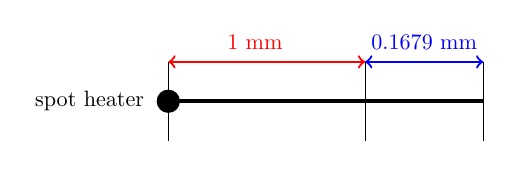
\begin{tikzpicture}[scale = 1]

\filldraw [black] (0,0) circle (4pt);
\draw [ultra thick] (0.0,0.0) -- (4.0,0);

\draw [thin] (2.5,-0.5) -- (2.5,0.5);
\draw [thin] (4.0,-0.5) -- (4.0,0.5);
\draw [thin] (0.0,-0.5) -- (0.0,0.5);

\draw [thick, <->, red] (0.0,0.5) -- (2.5,0.5);
\draw [thick, <->, blue] (2.5,0.5) -- (4.0,0.5);

\node[scale=0.8, color = black] at (-1.0,0.0) {spot heater};
\node[scale=0.8, color = red] at (1.1,0.75) {1 mm};
\node[scale=0.8, color = blue] at (3.25,0.75) {0.1679 mm};

\end{tikzpicture}
\caption{Schematic of 1D insulation modelling; simulation length as a sum of ground insulation (in red) and winding insulation (in blue) connected in series.}
\end{figure}

\begin{figure}[H]
\centering
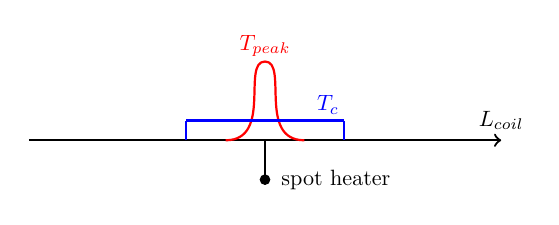
\begin{tikzpicture}[scale = 1]
\draw[thick, black, ->] (-3,0) -- (3,0);
\filldraw[black] (0,-0.5) circle (0.06);
\draw[thick, black] (0,0) -- (0,-0.5);
\draw [thick, red] (-0.5,0) .. controls +(0:0.6cm) and +(180:0.3cm) .. (0,1);
\draw [thick, red] (0,1) .. controls +(0:0.3cm) and +(180:0.6cm) .. (0.5,0);
\draw[thick, blue] (-1,0) -- (-1,0.25);
\draw[thick, blue] (-1,0.25) -- (1,0.25);
\draw[thick, blue] (1,0.25) -- (1,0);
\node[scale=0.8, black] at (0.9,-0.5) {spot heater};
\node[scale=0.8, black] at (3,0.25) {$L_\text{coil}$};
\node[scale=0.8, blue] at (0.8,0.45) {$T_\text{c}$};
\node[scale=0.8, red] at (0,1.2) {$T_\text{peak}$};
\end{tikzpicture}
\end{figure}

\begin{figure}[H]
\centering
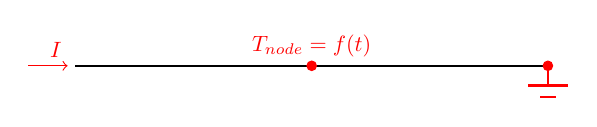
\begin{tikzpicture}[scale = 1]
\draw[thick, black] (-3,0) -- (3,0);
\filldraw[red] (3,0) circle (0.06);
\draw[thick, red] (3,0) -- (3,-0.25);
\draw[thick, red] (2.75,-0.25) -- (3.25,-0.25);
\filldraw[red] (0,0) circle (0.06);
\draw[thick, red] (2.9,-0.4) -- (3.1,-0.4);
\draw[thin, red, ->] (-3.6,0) -- (-3.1,0);
\node[scale=0.8, red] at (0,0.25) {$T_\text{node}= f(t)$};
\node[scale=0.8, red] at (-3.25,0.2) {$I$};
\end{tikzpicture}
\caption{Simulation settings}
\label{fig:sim_settings_3}
\end{figure}

\begin{figure}[H]
\centering
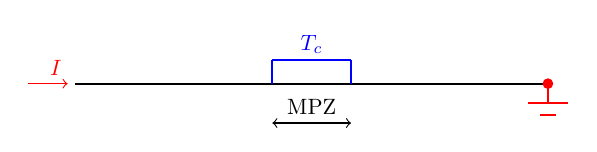
\begin{tikzpicture}[scale = 1]
\draw[thick, black] (-3,0) -- (3,0);
\filldraw[red] (3,0) circle (0.06);
\draw[thick, red] (3,0) -- (3,-0.25);
\draw[thick, red] (2.75,-0.25) -- (3.25,-0.25);
\draw[thick, red] (2.9,-0.4) -- (3.1,-0.4);
\draw[thin, red, ->] (-3.6,0) -- (-3.1,0);
\draw[thick, blue] (-0.5,0) -- (-0.5,0.3);
\draw[thick, blue] (-0.5,0.3) -- (0.5,0.3);
\draw[thick, blue] (0.5,0.3) -- (0.5,0);
\draw[thin, black, <->] (-0.5,-0.5) -- (0.5,-0.5);
\node[scale=0.8] at (0,-0.3) {MPZ};
\node[scale=0.8, blue] at (0,0.5) {$T_\text{c}$};
\node[scale=0.8, red] at (-3.25,0.2) {$I$};
\end{tikzpicture}
\caption{Simulation settings}
\label{fig:sim_settings_1}
\end{figure}

Until the quench is detected, the current inside the magnet is constant and equal to $I=86~\text{A}$. Therefore, the magnetic field inside the magnet does not vary in time. The analysis of steady-state magnetic field in the middle of the magnet for this value of current was conducted at INFN-Milano in OPERA software \cite{samuele_mariotto_mails}. A 2D interpolation had to be conducted in order to fit the OPERA mesh with the windings' position. For each winding, it is assumed that it is subjected to the magnetic field from the centre of its cross-section estimated by the interpolation map presented in Fig. \ref{fig:Quad_Mag_contour1}.
